% Options for packages loaded elsewhere
\PassOptionsToPackage{unicode}{hyperref}
\PassOptionsToPackage{hyphens}{url}
\PassOptionsToPackage{dvipsnames,svgnames,x11names}{xcolor}
%
\documentclass[
  letterpaper,
  DIV=11,
  numbers=noendperiod]{scrreprt}

\usepackage{amsmath,amssymb}
\usepackage{iftex}
\ifPDFTeX
  \usepackage[T1]{fontenc}
  \usepackage[utf8]{inputenc}
  \usepackage{textcomp} % provide euro and other symbols
\else % if luatex or xetex
  \usepackage{unicode-math}
  \defaultfontfeatures{Scale=MatchLowercase}
  \defaultfontfeatures[\rmfamily]{Ligatures=TeX,Scale=1}
\fi
\usepackage{lmodern}
\ifPDFTeX\else  
    % xetex/luatex font selection
\fi
% Use upquote if available, for straight quotes in verbatim environments
\IfFileExists{upquote.sty}{\usepackage{upquote}}{}
\IfFileExists{microtype.sty}{% use microtype if available
  \usepackage[]{microtype}
  \UseMicrotypeSet[protrusion]{basicmath} % disable protrusion for tt fonts
}{}
\makeatletter
\@ifundefined{KOMAClassName}{% if non-KOMA class
  \IfFileExists{parskip.sty}{%
    \usepackage{parskip}
  }{% else
    \setlength{\parindent}{0pt}
    \setlength{\parskip}{6pt plus 2pt minus 1pt}}
}{% if KOMA class
  \KOMAoptions{parskip=half}}
\makeatother
\usepackage{xcolor}
\setlength{\emergencystretch}{3em} % prevent overfull lines
\setcounter{secnumdepth}{5}
% Make \paragraph and \subparagraph free-standing
\makeatletter
\ifx\paragraph\undefined\else
  \let\oldparagraph\paragraph
  \renewcommand{\paragraph}{
    \@ifstar
      \xxxParagraphStar
      \xxxParagraphNoStar
  }
  \newcommand{\xxxParagraphStar}[1]{\oldparagraph*{#1}\mbox{}}
  \newcommand{\xxxParagraphNoStar}[1]{\oldparagraph{#1}\mbox{}}
\fi
\ifx\subparagraph\undefined\else
  \let\oldsubparagraph\subparagraph
  \renewcommand{\subparagraph}{
    \@ifstar
      \xxxSubParagraphStar
      \xxxSubParagraphNoStar
  }
  \newcommand{\xxxSubParagraphStar}[1]{\oldsubparagraph*{#1}\mbox{}}
  \newcommand{\xxxSubParagraphNoStar}[1]{\oldsubparagraph{#1}\mbox{}}
\fi
\makeatother


\providecommand{\tightlist}{%
  \setlength{\itemsep}{0pt}\setlength{\parskip}{0pt}}\usepackage{longtable,booktabs,array}
\usepackage{calc} % for calculating minipage widths
% Correct order of tables after \paragraph or \subparagraph
\usepackage{etoolbox}
\makeatletter
\patchcmd\longtable{\par}{\if@noskipsec\mbox{}\fi\par}{}{}
\makeatother
% Allow footnotes in longtable head/foot
\IfFileExists{footnotehyper.sty}{\usepackage{footnotehyper}}{\usepackage{footnote}}
\makesavenoteenv{longtable}
\usepackage{graphicx}
\makeatletter
\newsavebox\pandoc@box
\newcommand*\pandocbounded[1]{% scales image to fit in text height/width
  \sbox\pandoc@box{#1}%
  \Gscale@div\@tempa{\textheight}{\dimexpr\ht\pandoc@box+\dp\pandoc@box\relax}%
  \Gscale@div\@tempb{\linewidth}{\wd\pandoc@box}%
  \ifdim\@tempb\p@<\@tempa\p@\let\@tempa\@tempb\fi% select the smaller of both
  \ifdim\@tempa\p@<\p@\scalebox{\@tempa}{\usebox\pandoc@box}%
  \else\usebox{\pandoc@box}%
  \fi%
}
% Set default figure placement to htbp
\def\fps@figure{htbp}
\makeatother
% definitions for citeproc citations
\NewDocumentCommand\citeproctext{}{}
\NewDocumentCommand\citeproc{mm}{%
  \begingroup\def\citeproctext{#2}\cite{#1}\endgroup}
\makeatletter
 % allow citations to break across lines
 \let\@cite@ofmt\@firstofone
 % avoid brackets around text for \cite:
 \def\@biblabel#1{}
 \def\@cite#1#2{{#1\if@tempswa , #2\fi}}
\makeatother
\newlength{\cslhangindent}
\setlength{\cslhangindent}{1.5em}
\newlength{\csllabelwidth}
\setlength{\csllabelwidth}{3em}
\newenvironment{CSLReferences}[2] % #1 hanging-indent, #2 entry-spacing
 {\begin{list}{}{%
  \setlength{\itemindent}{0pt}
  \setlength{\leftmargin}{0pt}
  \setlength{\parsep}{0pt}
  % turn on hanging indent if param 1 is 1
  \ifodd #1
   \setlength{\leftmargin}{\cslhangindent}
   \setlength{\itemindent}{-1\cslhangindent}
  \fi
  % set entry spacing
  \setlength{\itemsep}{#2\baselineskip}}}
 {\end{list}}
\usepackage{calc}
\newcommand{\CSLBlock}[1]{\hfill\break\parbox[t]{\linewidth}{\strut\ignorespaces#1\strut}}
\newcommand{\CSLLeftMargin}[1]{\parbox[t]{\csllabelwidth}{\strut#1\strut}}
\newcommand{\CSLRightInline}[1]{\parbox[t]{\linewidth - \csllabelwidth}{\strut#1\strut}}
\newcommand{\CSLIndent}[1]{\hspace{\cslhangindent}#1}

\KOMAoption{captions}{tableheading}
\makeatletter
\@ifpackageloaded{bookmark}{}{\usepackage{bookmark}}
\makeatother
\makeatletter
\@ifpackageloaded{caption}{}{\usepackage{caption}}
\AtBeginDocument{%
\ifdefined\contentsname
  \renewcommand*\contentsname{Table of contents}
\else
  \newcommand\contentsname{Table of contents}
\fi
\ifdefined\listfigurename
  \renewcommand*\listfigurename{List of Figures}
\else
  \newcommand\listfigurename{List of Figures}
\fi
\ifdefined\listtablename
  \renewcommand*\listtablename{List of Tables}
\else
  \newcommand\listtablename{List of Tables}
\fi
\ifdefined\figurename
  \renewcommand*\figurename{Figure}
\else
  \newcommand\figurename{Figure}
\fi
\ifdefined\tablename
  \renewcommand*\tablename{Table}
\else
  \newcommand\tablename{Table}
\fi
}
\@ifpackageloaded{float}{}{\usepackage{float}}
\floatstyle{ruled}
\@ifundefined{c@chapter}{\newfloat{codelisting}{h}{lop}}{\newfloat{codelisting}{h}{lop}[chapter]}
\floatname{codelisting}{Listing}
\newcommand*\listoflistings{\listof{codelisting}{List of Listings}}
\makeatother
\makeatletter
\makeatother
\makeatletter
\@ifpackageloaded{caption}{}{\usepackage{caption}}
\@ifpackageloaded{subcaption}{}{\usepackage{subcaption}}
\makeatother

\usepackage{bookmark}

\IfFileExists{xurl.sty}{\usepackage{xurl}}{} % add URL line breaks if available
\urlstyle{same} % disable monospaced font for URLs
\hypersetup{
  pdftitle={LIMMMA Documentation},
  colorlinks=true,
  linkcolor={blue},
  filecolor={Maroon},
  citecolor={Blue},
  urlcolor={Blue},
  pdfcreator={LaTeX via pandoc}}


\title{LIMMMA Documentation}
\author{}
\date{2025-02-17}

\begin{document}
\maketitle

\renewcommand*\contentsname{Table of contents}
{
\hypersetup{linkcolor=}
\setcounter{tocdepth}{2}
\tableofcontents
}

\bookmarksetup{startatroot}

\chapter*{Preface}\label{preface}
\addcontentsline{toc}{chapter}{Preface}

\markboth{Preface}{Preface}

\bookmarksetup{startatroot}

\chapter*{Introduction}\label{introduction}
\addcontentsline{toc}{chapter}{Introduction}

\markboth{Introduction}{Introduction}

(Notes)

Biological, social and physical sciences -- community engaged. Landscape
change -- ecosystem services, well-being, livelihoods. Critical
transition zones -- impact of `sustainability' interventions.
Understanding use of different system framings and forms of
knowledge/evidence across scales. Decision making for resilient future
landscapes which support ecosystem services and wellbeing.

Understanding the changing function and value of multifunctional
landscapes and how they are shaped. Build up detailed multifunctional
landscape mosaic of social, cultural, biophysical and economic issues
associated with the suitability and impact of NbS/nature recovery.
(Connectivities, co-benefits, trade-offs) Strong contextual foundation
for utilizing emerging science from Nature Returns and others. Increased
involvement of local communities including citizen science. Sharing
lessons from NbS interventions over the long-term. Support and
contextualise NbS policy and plans and their evaluation. Gain real-time
feedback from policy interventions. Scale up lessons from pilot site
living labs.

\bookmarksetup{startatroot}

\chapter{Getting Started}\label{getting-started}

\section{Setting up a new project}\label{setting-up-a-new-project}

\begin{figure}[H]

{\centering \pandocbounded{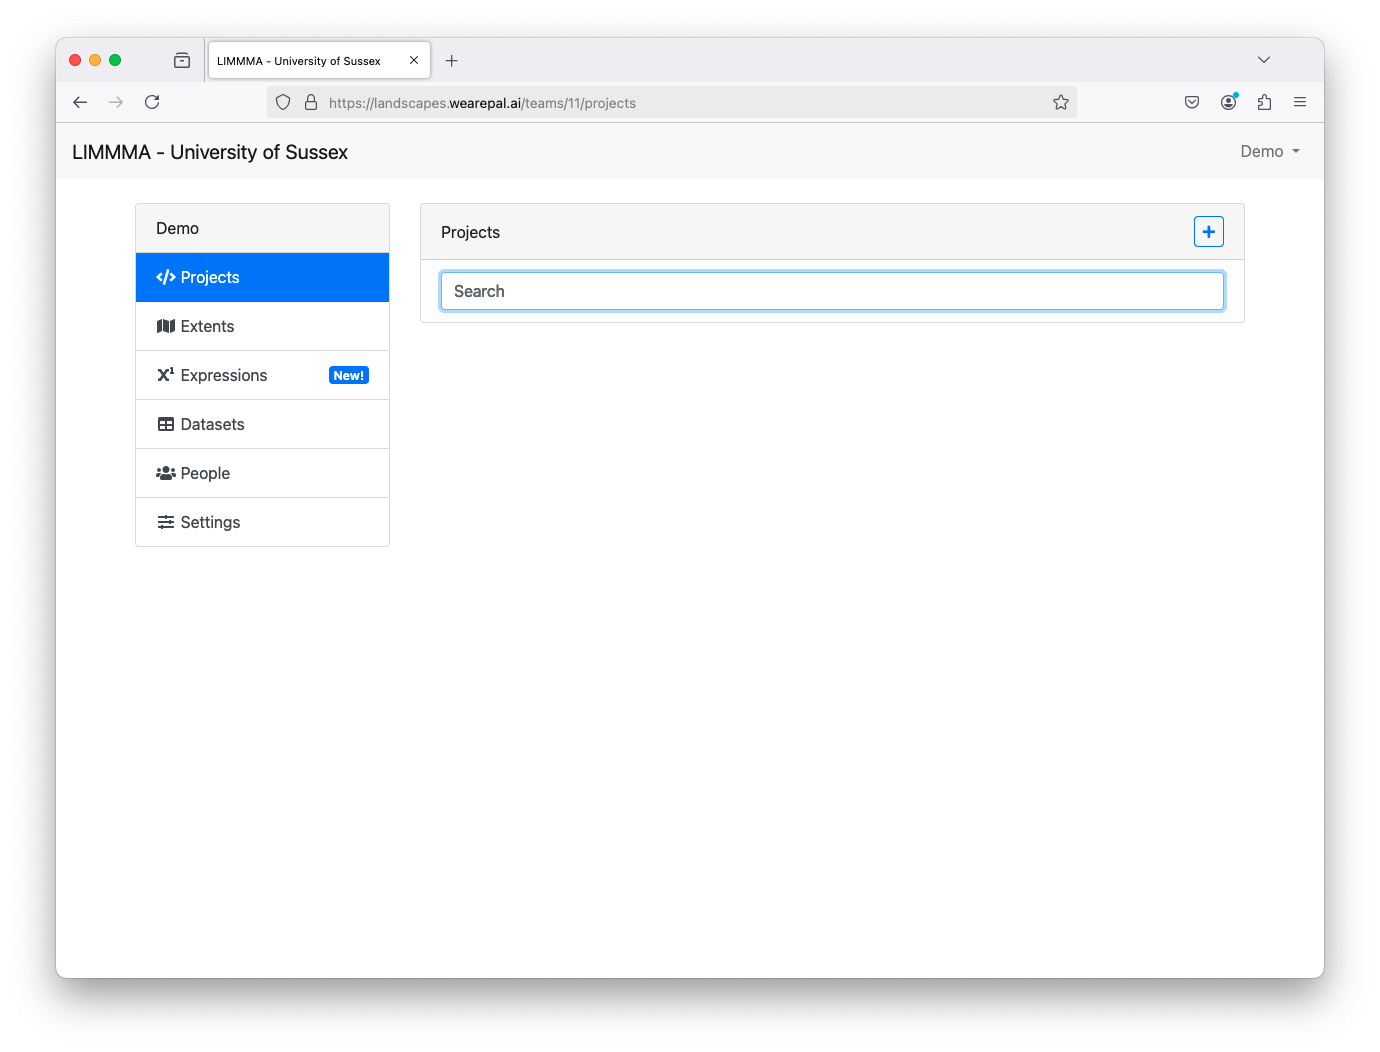
\includegraphics[keepaspectratio]{images/01-screenshots-start/01-01-Projects.png}}

}

\caption{Projects}

\end{figure}%%
\begin{figure}[H]

{\centering \pandocbounded{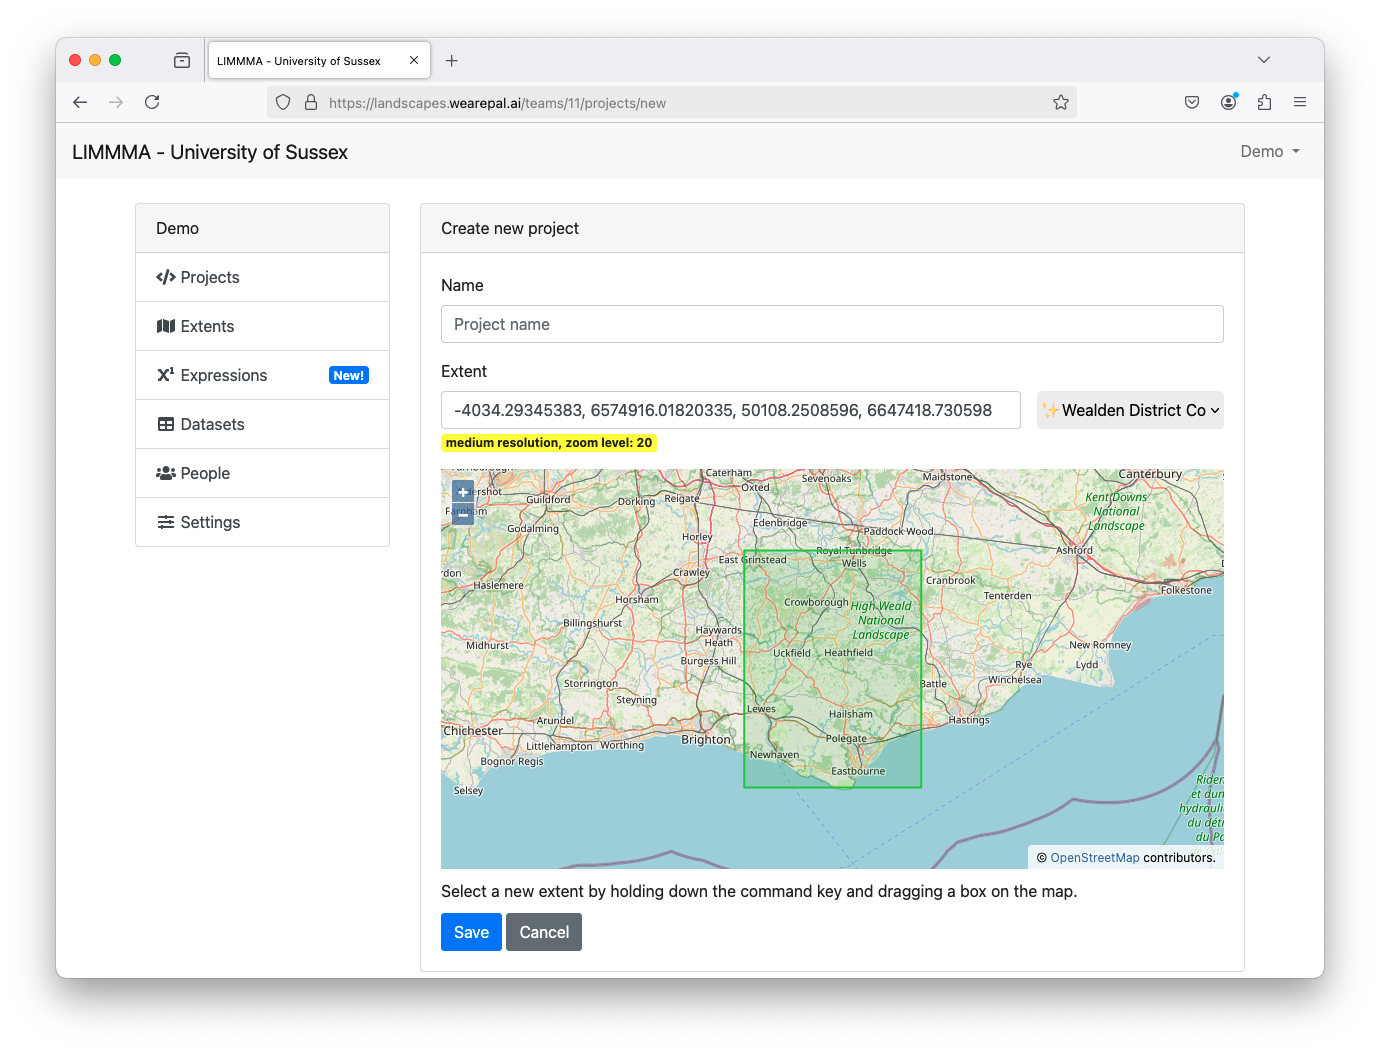
\includegraphics[keepaspectratio]{images/01-screenshots-start/01-02-Extent.png}}

}

\caption{Extent}

\end{figure}%

\subsection{Create an account}\label{create-an-account}

\subsection{Create a new project and set
extent}\label{create-a-new-project-and-set-extent}

\section{Map View}\label{map-view}

\subsection{Adding layers}\label{adding-layers}

\subsection{Snapshot tool}\label{snapshot-tool}

\section{Model View}\label{model-view}

\bookmarksetup{startatroot}

\chapter{Key Features}\label{key-features}

\bookmarksetup{startatroot}

\chapter{Use Case 1: Above Ground
Carbon}\label{use-case-1-above-ground-carbon}

As part of the Nature Returns research project with Natural England, the
LIMMMA team worked with Kew Wakehurst on landscape-based carbon storage
modelling. This involved using habitat maps, remote sensing data and
equations for estimating the amount of carbon stored above ground (in
vegetation such as trees and hedgerows) and below ground (in soils)
across a diverse landscape of woodland, grassland and built up areas at
different scales including 1) Wakehurst site, 2) Wealden District
Council, 3) Southeast England with potential to be scaled nationally.

In the following walkthrough we demonstrate how the above ground carbon
models were created and tested using LIMMMA.

\section{Basic Concepts}\label{basic-concepts}

If you are new to the idea of thinking about the landscape as a store of
carbon then there are a few basic concepts you need to understand before
we go any further. If you already know all about vegetative carbon and
soil carbon you can skip to the next section.

\subsection{Carbon Cycle}\label{carbon-cycle}

As an essential element of life, carbon is taken in, stored and released
by all living organisms. Through photosynthesis plants remove carbon
dioxide from the air, use the carbon to grow and release oxygen back
into the air. Although they also release carbon dioxide, over the course
of their life cycle, plants are net consumers of carbon. When they die
their carbon enters the soil. Some of this carbon becomes food for
organisms in the soil and makes its way back into the air, but, under
the right circumstances, a portion of it can remain there indefinitely.
Although the amount of carbon flowing through the vegetation and soil in
any landscape is constantly changing, given the right information we can
estimate a snapshot the total amount of carbon stored in the landscape
at a specific point in time and potentially predict the net impact of
that landscape on carbon emissions over a given period of time.

\subsection{Estimating Stored Carbon}\label{estimating-stored-carbon}

The first step towards making these kind of predictions is to estimate
the stock of carbon stored in the landscape and map its distribution
across space. Below is a visual illustration of the basic methods used
to make such estimates.

Imagine a landscape with a mixture of woodland, farmland, residential
areas and urban/sub-urban trees and other greenery.

\begin{figure}[H]

{\centering \pandocbounded{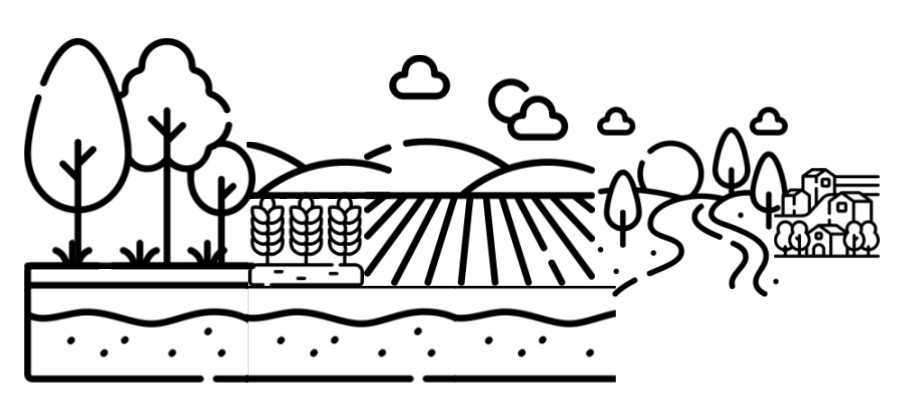
\includegraphics[keepaspectratio]{images/03-screenshots-agc/03-01-how-much-carbon.png}}

}

\caption{How much carbon is stored in this landscape?}

\end{figure}%

Above the ground, carbon is stored for long periods of time in large
areas of woodland, hedges and lone trees in agricultural fields as well
as individual trees in amongst buildings and roads. Arable crops and
wild grasslands store much smaller amounts of carbon for very short
periods of time until their carbon is either consumed by humans or
animals (to be released again to the air) or is gradually incorporated
into the soil as they decompose.

\begin{figure}[H]

{\centering \pandocbounded{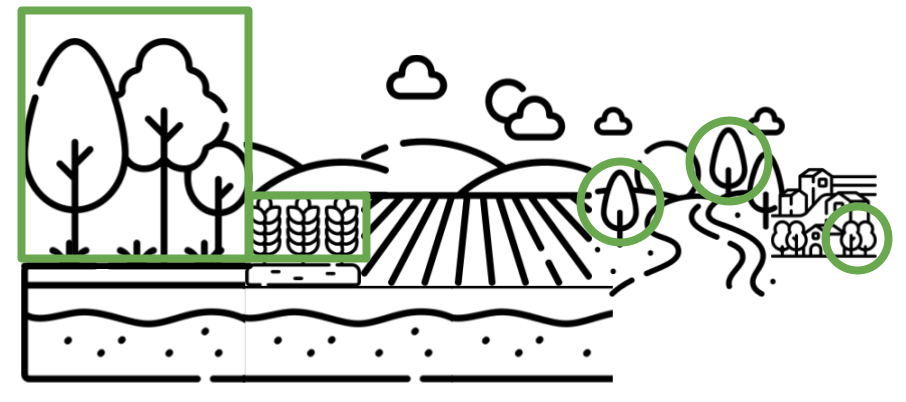
\includegraphics[keepaspectratio]{images/03-screenshots-agc/03-02-above-ground-carbon.png}}

}

\caption{Carbon stored above ground in vegetation}

\end{figure}%

Carbon in rotting plant matter from trees and other vegetation, once
incorporated into the soil becomes part of the soil-carbon-cycle and a
portion of it is stored for various periods of time. Under the right
conditions, the soil can accumulate a vast store of carbon which may
remain locked away for long periods of time. Taking account of above and
below ground carbon, over the course of 100 years a native broadleaf
woodland can store between 300 - 350 tonnes of carbon per
hectare.\footnote{https://www.woodlandtrust.org.uk/plant-trees/woodland-carbon-farmers-and-landowners/.}
If we convert that to an annual figure (3 - 3.5 tons) we can see that
this is roughly equal to 80\% of the average carbon footprint per person
in the UK (4.4 tons\footnote{https://ourworldindata.org/co2-and-greenhouse-gas-emissions.}).

\begin{figure}[H]

{\centering \pandocbounded{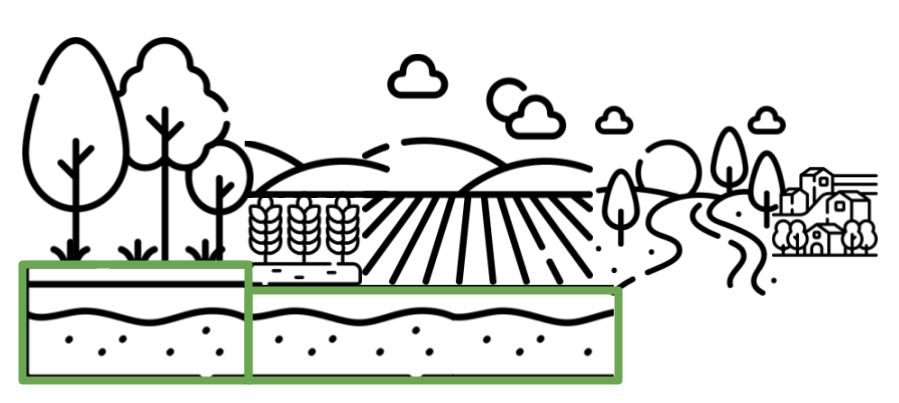
\includegraphics[keepaspectratio]{images/03-screenshots-agc/03-03-below-ground-carbon.png}}

}

\caption{Carbon stored below ground in soils}

\end{figure}%

The starting point for estimating the distribution of stored carbon in a
landscape is to classify it into different habitats (broadleaf woodland,
coniferous woodland, grassland, arable, etc.). Then we assign a fixed
estimate (based on field research) of the amount of carbon stored per
unit of each habitat.

\begin{figure}[H]

{\centering \pandocbounded{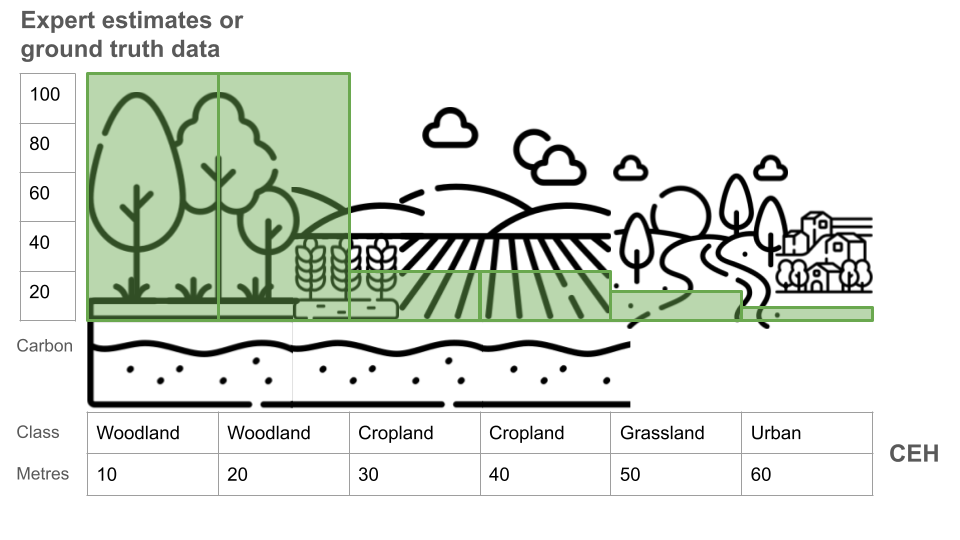
\includegraphics[keepaspectratio]{images/03-screenshots-agc/03-04-carbon-estimates.png}}

}

\caption{Estimating above ground carbon based on habitat
classifications}

\end{figure}%

Of course, within each habitat there are huge variations in the density
and height of vegetation as well as the quantity of carbon accumulated
in soils. These variations are not captured by a simple average per unit
of habitat. Additional data is needed to reflect within-habitat
variations, such as topography. Lidar measurements can give us an
estimate of the height of trees and other vegetation and some indication
of the density of vegetation. This data can then be used in equations to
estimate the total vegetative carbon distribution across a single
habitat such as broadleaved woodland. To supplement the habitat-based
estimates we can also use AI-assisted feature detection on satellite
imagery or areal imagery to identify lone trees or street trees which
would otherwise not be included in the habitat classifications.

Using LIMMMA we can make use of these different sources of data and try
out multiple combinations of data and methods for transforming them into
carbon density maps. The next section explains the different approaches
demonstrated in \ldots.

\section{Methodologies and Datasets}\label{methodologies-and-datasets}

Our aim in this project was to create a workflow for generating and
improving geospatial estimates of the amount of carbon stored above
ground in the natural landscape which met the following requirements:

\begin{enumerate}
\def\labelenumi{\arabic{enumi}.}
\tightlist
\item
  Use open access national datasets.
\item
  Scaleable from local to national.
\item
  Easily compare across different models at different scales.
\item
  Rapidly improve with new data, equations (e.g.~allometric) and
  methodologies as they emerge from ongoing research.
\end{enumerate}

The data and methods adopted are summarised in the following diagram.

\begin{figure}[H]

{\centering \pandocbounded{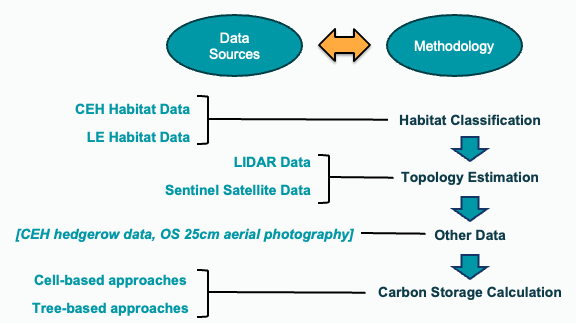
\includegraphics[keepaspectratio]{images/03-screenshots-agc/03-05-agc-data-methodology.png}}

}

\caption{Above Ground Carbon data and methodology}

\end{figure}%

Two options for generating the habitat basemap for carbon estimates were
imported: one from CEH and the other from LE. LIDAR and Sentinel
Satellite imagery provided the two options for topology estimation.
Additional data included CEH hedgerows and OS 25cm arial photography.
These data were variously used in different methods of carbon storage
calculation using a cell-based approach. The four methodologies listed
below build on each other iteratively to progress towards a more precise
estimate of carbon storage generated by increasingly complex models with
potential for continuous improvement.

\begin{figure}[H]

{\centering \pandocbounded{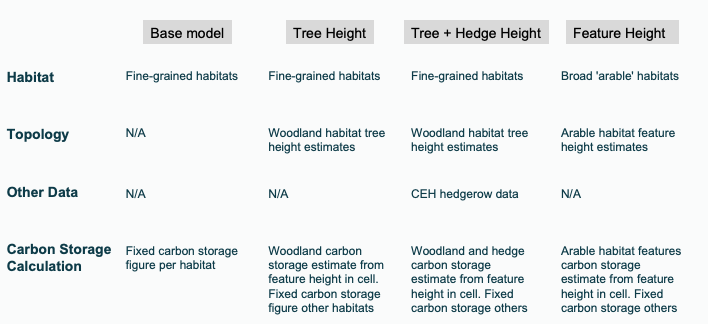
\includegraphics[keepaspectratio]{images/03-screenshots-agc/03-06-agc-methods-table.png}}

}

\caption{Above Ground Carbon evolving methodologies}

\end{figure}%

In the image below we can see how each model progressively improves the
fidelity of carbon estimate maps by variously increasing their
resolution and coverage.

\begin{figure}[H]

{\centering \pandocbounded{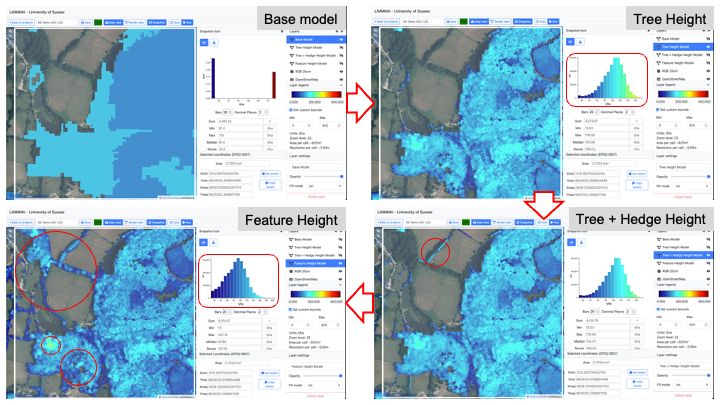
\includegraphics[keepaspectratio]{images/03-screenshots-agc/03-07-agc-progression.png}}

}

\caption{Above Ground Carbon model outputs showing increasing fidelity}

\end{figure}%

And here is an example of the outputs from the model in LIMMMA map view
at different scales.

\begin{figure}[H]

{\centering \pandocbounded{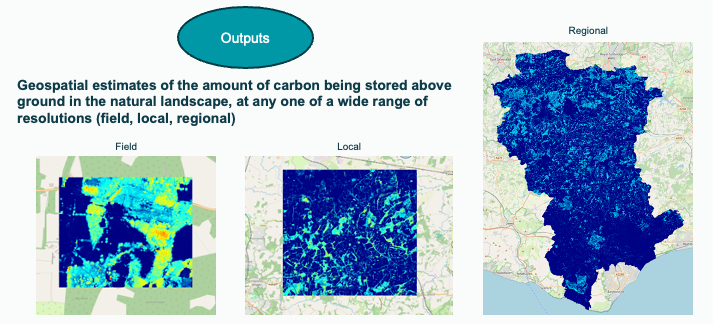
\includegraphics[keepaspectratio]{images/03-screenshots-agc/03-08-example-output.png}}

}

\caption{Example LIMMMA outputs}

\end{figure}%

The following section describes how each of these models was built and
how the outputs were created and analysed to draw conclusions about the
different levels and sources of uncertainty associated with each.

\section{Implementing models}\label{implementing-models}

Each model was built in LIMMMA's graphical modelling system. The
following diagram shows how it is used to connect data, methods and
outputs in a single visual interface.

\begin{figure}[H]

{\centering \pandocbounded{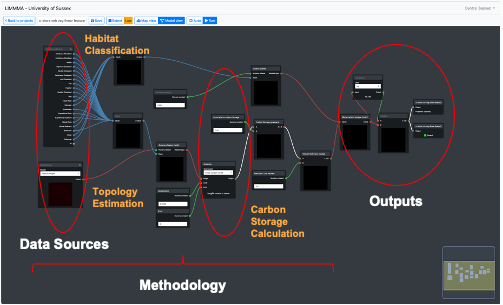
\includegraphics[keepaspectratio]{images/03-screenshots-agc/03-09-example-model.png}}

}

\caption{Example LIMMMA model}

\end{figure}%

Having created a new project and set our desired extent, we can open the
model view and start building. At first, you will be presented with a
blank screen with no visible controls. Don't worry, the first thing to
do is to add the data components that you want to include in your model.
This is done by simply right clicking the screen and selecting from a
list of whatever datasets you have already imported into you team's
workspace in the LIMMMA app.

\subsection{Select datasets}\label{select-datasets}

\subsection{Transform data}\label{transform-data}

\subsection{Generate outputs}\label{generate-outputs}

\section{Exploring outputs}\label{exploring-outputs}

\bookmarksetup{startatroot}

\chapter{Use Case 2: Below Ground
Carbon}\label{use-case-2-below-ground-carbon}

\bookmarksetup{startatroot}

\chapter{Use Case 3: Multifunctional Landscape
Analysis}\label{use-case-3-multifunctional-landscape-analysis}

\bookmarksetup{startatroot}

\chapter{Use Case 4: AI Supported Land-Use
Classification}\label{use-case-4-ai-supported-land-use-classification}

\bookmarksetup{startatroot}

\chapter*{References}\label{references}
\addcontentsline{toc}{chapter}{References}

\markboth{References}{References}

\phantomsection\label{refs}
\begin{CSLReferences}{0}{1}
\end{CSLReferences}

\bookmarksetup{startatroot}

\chapter{Habits}\label{habits}

\bookmarksetup{startatroot}

\chapter{In the morning}\label{in-the-morning}

\section{Getting up}\label{getting-up}

\begin{itemize}
\tightlist
\item
  Turn off alarm
\item
  Get out of bed
\end{itemize}

\section{Breakfast}\label{breakfast}

\begin{itemize}
\tightlist
\item
  Eat eggs
\item
  Drink coffee
\end{itemize}

\bookmarksetup{startatroot}

\chapter{In the evening}\label{in-the-evening}

\section{Dinner}\label{dinner}

\begin{itemize}
\tightlist
\item
  Eat spaghetti
\item
  Drink wine
\end{itemize}

\section{Going to sleep}\label{going-to-sleep}

\begin{itemize}
\tightlist
\item
  Get in bed
\item
  Count sheep
\end{itemize}




\end{document}
